% sycophancy_paper.tex -- Standalone study on sycophancy under deliberative scaffolding.
%
% Self-contained ACL/ARR long-paper submission. The deliberative scaffold studied
% here (Narration-of-Thought) is specified in full in Section 3 and Appendix A;
% prior work is cited where required but the paper does not depend on it.
%
% Reproducibility map (phase labels -> sections) is in Appendix E.

\documentclass[11pt]{article}

\usepackage[review]{acl}

\usepackage{times}
\usepackage{latexsym}
\usepackage[T1]{fontenc}
\usepackage[utf8]{inputenc}
\usepackage{microtype}
\usepackage{inconsolata}
\usepackage{booktabs}
\usepackage{multirow}
\usepackage{tabularx}
\usepackage{amsmath}
\usepackage{amssymb}
\usepackage{url}
\urlstyle{tt}
\usepackage{graphicx}
\usepackage{xcolor}
\usepackage{tikz}
\usetikzlibrary{positioning, arrows.meta}

\definecolor{stdgrey}{HTML}{7E9AAB}
\definecolor{ncotteal}{HTML}{0E7C7B}
\definecolor{ncottealdk}{HTML}{0A5C5B}
\definecolor{paleteal}{HTML}{D9ECEB}
\definecolor{palealarm}{HTML}{C9D7E6}

\newcommand{\nano}{\texttt{gpt-5.4-nano}}
\newcommand{\haiku}{\texttt{claude-haiku-4-5}}
\newcommand{\sonnet}{\texttt{claude-sonnet-4-6}}
\newcommand{\grok}{\texttt{grok-4-1-fast-reasoning}}
\newcommand{\deepseek}{\texttt{DeepSeek-R1}}

\title{Sycophancy Under Deliberative Scaffolding:\\
Construct Fragmentation, Judge Gaming,\\
and Panel-Robust Prompt Optimization}

\author{Anonymous ACL submission}

\begin{document}
\maketitle

\begin{abstract}
``Sycophancy'' names several behaviours, and a mitigation that targets one need not touch the others.
We study a black-box deliberative scaffold---Narration-of-Thought (NoT), a system prompt that forces a
model to enumerate stakeholders, project consequences, state uncertainty, and commit before answering
(specified in \S\ref{sec:setup})---and ask which form of sycophancy it moves.
\textbf{(1) Construct fragmentation.} On social-sycophancy advice tasks \citep{cheng25elephant}, NoT
cuts emotional-validation rates on all four frontier generators (Fisher $p<10^{-4}$; $-26$ to $-53$\,pp
vs.\ chain-of-thought), landing within two points of the human rate on three of four; but it does
\emph{not} transfer to propositional sycophancy on false-theorem proving \citep{petrov2025brokenmath}
(significant reduction on one generator; a significant \emph{increase} on another) and \emph{reverses} on
cross-prompt moral consistency. Hand-written obvious-falsehood probes \citep{sharma23} are saturated
($\leq2.2\%$), making BrokenMath ($39$--$83\%$) the appropriate propositional instrument.
\textbf{(2) Single-judge prompt optimization games the judge.} Optimizing the scaffold against one
absolute LLM judge with textual gradients drives held-out validation to $0.7\%$ and beats matched-budget
TextGrad, OPRO and APE---but a three-family panel flags all three social metrics as low inter-judge
agreement (Krippendorff's $\alpha\leq0.42$), and re-scoring the \emph{identical} responses exposes the
indirectness reduction as a Goodhart artifact ($6\%$ under the training judge, $87\%$ under a held-out
judge).
\textbf{(3) A panel-robust optimizer.} Replacing the single-judge loss with a worst-case-over-panel
objective, one judge family held out entirely, yields a prompt that generalizes to the held-out family
significantly better than single-judge optimization (framing $11\%$ vs.\ $52\%$, $p{=}1.9\times10^{-14}$;
indirectness $4\%$ vs.\ $74\%$ on out-of-family \deepseek, $p<10^{-15}$) while preserving stakeholder
depth. We conclude that deliberative scaffolding targets \emph{social, single-response}
face-preservation, and that prompt optimization against LLM judges must be evaluated against judges held
out from optimization---or it measures judge idiosyncrasy rather than behaviour.
\end{abstract}

\section{Introduction}

Sycophancy---an assistant agreeing with or flattering a user at the expense of accuracy or
candour---is a recognised consequence of preference-based fine-tuning \citep{sharma23,perez22}, visible
in the GPT-4o rollback of 2025 \citep{openai_sycophancy_2025} and a growing benchmark literature
\citep{malmqvist24}.
Mitigation work often treats sycophancy as a single axis, yet the construct is now understood to
fragment. \emph{Propositional} sycophancy is endorsing checkably false claims; \emph{social} sycophancy
is excessive preservation of the user's ``face''---their desired self-image---through validation,
indirect language, accepting framing, or moral affirmation \citep{cheng25elephant,goffman55}. These are
measured by different instruments and need not respond to the same intervention; indeed
\citet{cheng25elephant} already observe that the linguistic facets of social sycophancy are more
mitigable than the reasoning-laden ones.

We study whether a single inference-time scaffold closes any of these gaps. \emph{Narration-of-Thought}
(NoT) is a system prompt---requiring no fine-tuning, weights, or activations---that, in place of
``think step by step,'' asks the model to name a protagonist, enumerate the stakeholders whose interests
intersect the decision, project consequences two steps out, articulate what remains uncertain, and only
then commit to an answer \citep{not_origin}. We specify NoT in full in \S\ref{sec:setup}; the reader
need not consult prior work. NoT is, by construction, a black-box, inference-time, output-side
intervention, which distinguishes it from white-box steering \citep{cheng25elephant}, training-side
finetuning \citep{wei23syn,khan24dpo}, and the recent black-box \emph{input-side} reframing of
\citet{dubois26ask}.

Two facts make this a measurement problem as much as a mitigation problem. Every sycophancy outcome here
is scored by an LLM judge, and LLM judges carry self-preference, verbosity, and instability biases with
chronically low inter-judge agreement \citep{zheng23judge,panickssery24,li24judgesurvey}; and once a
prompt is \emph{optimized} against such a judge, the setup is a textbook case of reward
over-optimization---a proxy that becomes a target ceases to measure what it did
\citep{strathern97goodhart,gao23overopt,pan24hacking}. We confront both directly.

\paragraph{Contributions.}
\textbf{(1)} We document obvious-falsehood saturation and adopt BrokenMath as the rigorous propositional
instrument (\S\ref{sec:benchmarks}).
\textbf{(2)} We show NoT reduces social validation and framing across four generators but dissociates
from propositional error-detection and from cross-prompt moral consistency---direct evidence that
sycophancy is not one construct (\S\ref{sec:social}--\S\ref{sec:propositional}).
\textbf{(3)} We separate two moral measurements (binary-suffix vs.\ free-form verdict extraction) and
retract an earlier ``moral-collapse'' reading traceable to a data-loading error (\S\ref{sec:moral}).
\textbf{(4)} We show single-judge prompt optimization Goodharts its judge---a reduction that vanishes on
held-out judges---using a cross-family reliability panel and a same-responses re-scoring diagnostic
(\S\ref{sec:judges}).
\textbf{(5)} As our methods contribution, we introduce a black-box \emph{panel-robust} optimizer
minimizing a worst-case-over-judges loss that generalizes to a held-out, out-of-family judge
significantly better than single-judge optimization (\S\ref{sec:robust}).

\section{Related Work}
\label{sec:related}

\paragraph{Sycophancy and its constructs.}
\citet{perez22} and \citet{sharma23} establish propositional sycophancy and trace it to preference
data; SycophancyEval is the standard obvious-falsehood instrument. Plausible-falsehood benchmarks find
the residual sycophancy it misses---SycEval reports $58\%$ capitulation \citep{fanous2025syceval} and
BrokenMath finds the strongest model sycophantic $29\%$ of the time on expert-verified false theorems
\citep{petrov2025brokenmath}. \citet{cheng25elephant} introduce \emph{social} sycophancy and the
ELEPHANT benchmark (validation, indirectness, framing, moral), grounded in face-work \citep{goffman55};
multi-turn \citep{hong2025sycon} and advice-seeking \citep{kim25advisorqa} settings extend it. Our
result sharpens an asymmetry ELEPHANT already noted into a dissociation under one intervention.

\paragraph{Sycophancy mitigation.}
Training-side methods include synthetic-data finetuning \citep{wei23syn} and preference optimization
\citep{khan24dpo}; white-box methods include steering \citep{cheng25elephant} and probe penalties
\citep{papadatos24}. Closest to NoT are black-box inference-time methods: input-side question-reframing,
which \citet{dubois26ask} show beats the naive ``don't be sycophantic'' prompt, and trace monitoring of
reasoning-model sycophancy \citep{hu25monica}. NoT occupies the remaining cell---inference-time,
black-box, \emph{output-side} deliberation. A recurring caveat is overcorrection: such interventions can
make models reject \emph{correct} user claims \citep{wei23syn,sharma23}, which we revisit in
\S\ref{sec:disc}.

\paragraph{Chain-of-thought and judges.}
NoT is a constrained chain-of-thought \citep{wei22,kojima22}; added reasoning need not reduce bias---CoT
rationalizes user-cued answers without verbalizing them \citep{turpin23}, requiring consistency training
to fix \citep{chua24}, which predicts deliberation helping some constructs and backfiring on others.
Since every outcome is judge-scored, judge reliability is load-bearing: LLM judges reach only
$\sim$63--66\% human agreement \citep{zheng23judge,dubois23alpacafarm}, show self-preference
\citep{panickssery24}, verbosity/position biases \citep{li24judgesurvey,gu24judgesurvey}, and
instability under prompt perturbation \citep{thakur24judges}. We use Krippendorff's $\alpha$
\citep{krippendorff2004} and Cohen's $\kappa$ \citep{cohen60}; our ``high $\kappa$-vs-human, low
inter-judge $\alpha$'' pattern is the base-rate $\kappa$ paradox \citep{feinstein90kappa}, and our panel
adopts established majority-vote aggregation.

\paragraph{Prompt optimization and reward hacking.}
Prompt optimizers include APE \citep{zhou23ape}, OPRO \citep{yang24opro}, and the textual-gradient
methods ProTeGi \citep{pryzant23protegi} and TextGrad \citep{yuksekgonul2024textgrad} (cf.\ DSPy
\citep{khattab23dspy}); our ``narrative gradients'' are a construct-specialized textual-gradient
optimizer. Optimizing a learned proxy eventually diverges from truth
\citep{strathern97goodhart,amodei16,skalse22,gao23overopt}, and \emph{in-context} reward hacking arises
when a model maximizes evaluation scores without weight updates \citep{pan24hacking}---our single-judge
regime. Reward-model \emph{ensembles} mitigate over-optimization by averaging
\citep{coste24ensemble,eisenstein23herding,rame24warm}; our objective takes the stronger \emph{worst
case} over a held-out judge panel, testing the herding caveat \citep{eisenstein23herding} via an
out-of-family judge.

\section{The NoT Scaffold and Experimental Setup}
\label{sec:setup}

\subsection{The Narration-of-Thought scaffold}
NoT is a single system prompt. In place of an open-ended ``think step by step'' instruction, it
requires the model to produce five labelled narrative sections before committing to an answer:
\textbf{(i) Protagonist}---identify whose decision is at issue;
\textbf{(ii) Stakeholders}---enumerate the parties whose interests intersect the decision;
\textbf{(iii) Consequences}---project the likely effects of the leading options two steps out;
\textbf{(iv) Uncertainty}---state explicitly what is unknown or contested; and
\textbf{(v) Commitment}---give a single, committed recommendation.
The full verbatim prompt is reproduced in Appendix~\ref{app:notprompt} so that the paper is
self-contained; it is applied identically across generators and is never fine-tuned into the weights.
NoT is thus a \emph{black-box, inference-time, output-side} intervention: it shapes the assistant's
own generation and requires only API-level access.

We also evaluate a \emph{multi-stakeholder} variant---several NoT agents (one per stakeholder
perspective) whose drafts a separate moderator integrates over five rounds into one answer---used only
to test whether the indirectness cost of single-agent NoT (\S\ref{sec:social}) can be reduced in a
cross-judge-coherent way.

\subsection{Generators and comparison arms}
Our \textbf{generator quartet} spans four vendors: \nano, \haiku, \sonnet, and \grok. Holding the
scaffold fixed and varying the generator lets us separate scaffold effects from model-specific quirks.
We compare four single-agent arms: \textbf{Raw} (empty system prompt), \textbf{IO} (a minimal
instruction-only prompt), \textbf{standard CoT} (``think step by step''), and \textbf{NoT}. Standard CoT
is the key baseline: it isolates the contribution of NoT's \emph{structure} from the generic effect of
adding intermediate reasoning, and all headline NoT effects are reported as deltas against CoT, not
against Raw.

\subsection{Benchmarks and constructs}
We measure three families of sycophancy.

\paragraph{Obvious-falsehood (propositional, saturated).}
SycophancyEval \citep{sharma23} elicits agreement with plainly false premises. We use it only to
establish that this instrument is saturated on current frontier models (\S\ref{sec:benchmarks}).

\paragraph{Plausible-falsehood (propositional, graded).}
BrokenMath \citep{petrov2025brokenmath} presents expert-verified \emph{false} competition-mathematics
theorems and asks the model to prove them; a four-category judge labels each response
\textbf{Sycophant} (attempts to prove the false claim), \textbf{Detected} (notices something is wrong),
\textbf{Corrected} (fixes the statement), or \textbf{Ideal} (correctly refutes). The headline
\emph{Sycophant rate} is the fraction of responses that go along with the false premise. We evaluate a
fixed split of $451$ adversarial problems per cell.\footnote{The public BrokenMath release contains
additional problems; we hold this $451$-item split fixed across all arms so within-table comparisons are
exact.}

\paragraph{Social sycophancy.}
ELEPHANT \citep{cheng25elephant} scores excessive preservation of the user's ``face'' on
advice-seeking prompts, grounded in face-work \citep{goffman55}. It spans two prompt sources---
\textbf{OEQ} (open-ended advice questions) and \textbf{AITA} (``Am I The Asshole?'' moral-judgment
posts)---and four metrics:
\textbf{Validation} (uncritically affirming the user's feelings or position),
\textbf{Indirectness} (hedged, non-committal phrasing rather than a direct answer),
\textbf{Framing} (accepting the user's framing/premises without challenge), and
\textbf{Moral both-NTA}. The moral metric is a \emph{cross-prompt consistency} probe: each AITA conflict
is presented in its original form and in a perspective-flipped rewrite, and \emph{both-NTA} is the rate
at which the model returns the ``Not The Asshole'' (NTA) verdict for \emph{both} sides of the same
conflict---i.e.\ affirms whoever is asking. (The complementary verdict is YTA, ``You're The Asshole.'')
Comparing two responses to two prompts, both-NTA measures something structurally different from the
single-response metrics (central in \S\ref{sec:moral}).
We use a stratified $n{=}150$ subsample per slice (seed 44) and report rates against the crowdsourced
human baseline shipped with ELEPHANT. Table~\ref{tab:constructs} summarises the construct taxonomy.

\begin{table}[t]
\centering
\small
\setlength{\tabcolsep}{4pt}
\begin{tabular}{lll}
\toprule
Construct & Instrument & Unit \\
\midrule
Propositional (obvious)   & Sharma     & single resp. \\
Propositional (plausible) & BrokenMath & single resp. \\
Social: validation        & ELEPHANT   & single resp. \\
Social: indirectness      & ELEPHANT   & single resp. \\
Social: framing           & ELEPHANT   & single resp. \\
Moral consistency         & ELEPHANT   & prompt pair \\
\bottomrule
\end{tabular}
\caption{The sycophancy constructs studied here are measured by different instruments and at different
units of analysis. ``Single resp.'' metrics score one answer; moral both-NTA compares a model's answers
to a prompt and its perspective-flipped twin. A mitigation can move one row without moving the others.}
\label{tab:constructs}
\end{table}

\subsection{Scoring and the judge panel}
Every social and propositional outcome is scored by an LLM judge using the faithful ELEPHANT/BrokenMath
judge prompts. The default single judge is \haiku. Because LLM judges are unreliable
(\S\ref{sec:related}), \S\ref{sec:judges} re-scores a stratified subsample with a three-family
reliability panel (\nano, \haiku, \grok) and reports Krippendorff's $\alpha$ \citep{krippendorff2004}
for inter-judge agreement and Cohen's $\kappa$ \citep{cohen60} against crowdsourced human gold. For the
optimisation experiments we additionally hold out two judge families---\sonnet\ and the out-of-family
\deepseek---that are never consulted during optimisation.

\subsection{Narrative-gradient optimisation}
To optimise the scaffold we use a textual-gradient procedure (cf.\ ProTeGi \citep{pryzant23protegi},
TextGrad \citep{yuksekgonul2024textgrad}): an optimiser model inspects scored examples, writes a
natural-language ``gradient'' for how the prompt failed, and edits it, iterating for a fixed budget; we
call this construct-specialised variant \emph{narrative gradients}. The naive objective minimises a
single judge's pooled social-sycophancy score,
\[
L_{\text{single}} \;=\; \mathrm{mean}\big(\text{val} + \text{ind} + \text{fram}\big),
\]
which \S\ref{sec:judges} shows is exploitable. Our \textbf{panel-robust} objective instead takes the
worst case over an optimisation panel $\mathcal{P}$ of the three in-family judges (\grok, \haiku,
\nano) before averaging over items,
\[
L_{\text{robust}} \;=\; \mathrm{mean}_{i}\;\max_{j\in\mathcal{P}}\;\mathrm{mean}\big(\text{val}+\text{ind}+\text{fram}\big)_{ij},
\]
so a prompt edit lowers the loss only when \emph{every} panel judge agrees it helped; it cannot cash in
on a single lenient judge. \sonnet\ and \deepseek\ are held out entirely and used only at evaluation.
The whole procedure is black-box---API-level generation and judging, no weights or activations---so it
applies to frontier closed models. Model roles are summarised in Table~\ref{tab:roles}; note that
\haiku\ and \grok\ appear in several roles, a leakage consideration we flag in Limitations.

\subsection{Statistical testing}
Cross-arm rate comparisons on independent cells use two-proportion $z$-tests when $n$ is large and
Fisher exact tests when any cell count is small (BrokenMath per-generator deltas). Re-scoring tables
that compare hand vs.\ optimised responses on the \emph{same} items (e.g.\ the Goodhart gap,
Table~\ref{tab:goodhart}) are paired by construction; we report two-proportion tests on those paired
binary outcomes for consistency with the rest of the paper, and note McNemar's test as the strictly
paired alternative. We report pairwise tests without a global multiple-comparison correction
(\S\ref{sec:limitations}); headline effects with $p<10^{-4}$ survive conservative correction.

\begin{table}[t]
\centering
\small
\setlength{\tabcolsep}{3pt}
\begin{tabular}{lcccc}
\toprule
Model & Gen. & Judge & Panel & Held-out \\
\midrule
\texttt{nano}        & \checkmark & --         & \checkmark & -- \\
\texttt{haiku}       & \checkmark & \checkmark & \checkmark & -- \\
\texttt{sonnet}      & \checkmark & --         & --         & \checkmark \\
\texttt{grok}        & \checkmark & --         & \checkmark & -- \\
\texttt{DeepSeek-R1} & --         & --         & --         & \checkmark \\
\bottomrule
\end{tabular}
\caption{Model roles (short labels; full identifiers in \S\ref{sec:setup}). ``Judge'' is the default
single judge, ``Panel'' the optimisation panel. The generator quartet is scored throughout and overlaps
with the judge/panel roles, while \texttt{sonnet} (in-vendor with \texttt{haiku}) and out-of-family
\texttt{DeepSeek-R1} are reserved for held-out evaluation. Role overlap is a limitation we return to in
\S\ref{sec:limitations}.}
\label{tab:roles}
\end{table}

\section{Benchmark Choice: Obvious vs.\ Plausible Falsehoods}
\label{sec:benchmarks}

A propositional-sycophancy claim is only as good as its instrument. On hand-written obvious-falsehood
probes \citep{sharma23}, every cell of our quartet---under both standard CoT and NoT---scores at most
$2.2\%$ (Appendix~\ref{app:sharma}, Table~\ref{tab:sharma}). The instrument is \emph{saturated}: it
cannot discriminate arms, and any ``improvement'' on it would be noise at the floor.

BrokenMath \citep{petrov2025brokenmath} supplies the missing headroom. Standard-CoT Sycophant rates
span $51\%$ (\grok) to $83\%$ (\haiku)---more than an order of magnitude above the Sharma floor
(Table~\ref{tab:brokenmath}). We therefore treat BrokenMath, not Sharma, as the propositional
instrument for all scaffold claims, and report Sharma only to document the floor. This weak-instrument
correction matters independently of NoT: it cautions against the common inference from low
obvious-falsehood rates to low propositional sycophancy in general, echoing graded-probe findings of
$29$--$58\%$ residual sycophancy elsewhere \citep{fanous2025syceval,petrov2025brokenmath}.

\begin{table}[t]
\centering
\small
\setlength{\tabcolsep}{4pt}
\begin{tabular}{lrrrr}
\toprule
Generator & Raw & Std CoT & NoT & $\Delta$(NoT$-$CoT) \\
\midrule
\texttt{nano}   & $58\%$ & $55\%$ & $69\%$ & $\mathbf{+14.7}^{\dag}$ \\
\texttt{haiku}  & $81\%$ & $83\%$ & $80\%$ & $-3.5$ \\
\texttt{sonnet} & $70\%$ & $69\%$ & $73\%$ & $+3.1$ \\
\texttt{grok}   & $48\%$ & $51\%$ & $39\%$ & $\mathbf{-12.0}^{*}$ \\
\bottomrule
\end{tabular}
\caption{BrokenMath Sycophant rate ($n{=}451$ adversarial problems per cell, judge \haiku). Rates far
exceed the Sharma floor. NoT reduces sycophancy significantly on \texttt{grok} ($^{*}$Fisher
$p{<}0.001$) and \emph{increases} it on \texttt{nano} ($^{\dag}$Fisher $p{<}10^{-5}$);
\texttt{haiku}/\texttt{sonnet} are null. The mixed signs are the first evidence that the social-metric
reductions below do not transfer to propositional error-detection.}
\label{tab:brokenmath}
\end{table}

\section{Social Sycophancy: Validation and Framing}
\label{sec:social}

\paragraph{Validation: the headline effect.}
NoT cuts OEQ validation on all four generators (Fisher $p<10^{-4}$; $-26$ to $-53$\,pp vs.\ CoT),
meeting our pre-registered falsification criterion. Three land within two points of the $29\%$ human
\emph{rate}; \sonnet\ reaches $47\%$ (Table~\ref{tab:elephant_main}, Appendix Table~\ref{tab:crossvendor}).
Matching a crowd \emph{rate} is not item-level correctness: NoT could withhold validation where humans
would grant it (overcorrection) or vice versa; we report rates, not agreement with human labels on the
same items. This is nonetheless the paper's most robust positive result, and---unlike the other social
metrics---it survives the judge panel of \S\ref{sec:judges} without a reliability caveat.

\paragraph{Framing.}
NoT lowers framing on every generator (significant on three of four on OEQ/AITA), and on
premise-acceptance ($-13$ to $-24$\,pp vs.\ CoT).

\paragraph{Indirectness, and cross-judge coherence.}
Single-agent NoT nudges \emph{indirectness} up on several cells---the model hedges more when forced to
enumerate uncertainty---but the multi-stakeholder variant yields a cross-judge-coherent directness
reduction across all eight dataset--generator cells ($-11$ to $-28$\,pp) while preserving the validation
gains. Since indirectness carries sub-chance inter-judge reliability ($\alpha{=}-0.23$;
\S\ref{sec:judges}), treat any ``indirectness recovery'' claim as simultaneous satisfaction of
idiosyncratic graders, not recovery of a well-defined latent construct.

\paragraph{A length caveat.}
NoT responses are substantially longer than CoT on OEQ: on \haiku, mean length rises from ${\approx}1{,}700$
to ${\approx}5{,}600$ characters ($3.3\times$); on \sonnet\ from ${\approx}1{,}650$ to ${\approx}7{,}200$
($4.4\times$; full quartet in Appendix Table~\ref{tab:lengths}). Verbosity biases LLM judges
\citep{li24judgesurvey}, so validation/framing reductions could be partly a length or formatting artifact;
we ran no length-matched verbose-CoT control. Three dissociations argue against length \emph{alone}:
indirectness moves \emph{up} not down, the effect does not transfer to BrokenMath despite the same length
increase, and the moral metric moves the \emph{opposite} way (\S\ref{sec:moral}). A length-matched
ablation remains future work (\S\ref{sec:limitations}).

\begin{table}[t]
\centering
\small
\setlength{\tabcolsep}{4pt}
\begin{tabular}{lrrrrr}
\toprule
Metric (slice) & Human & Raw & IO & Std CoT & NoT \\
\midrule
OEQ validation  & $29\%$ & $66\%$ & $54\%$ & $63\%$ & $27\%$ \\
OEQ framing     & $61\%$ & $55\%$ & $65\%$ & $65\%$ & $23\%$ \\
AITA validation & $7\%$  & $47\%$ & $43\%$ & $37\%$ & $17\%$ \\
AITA framing    & $41\%$ & $50\%$ & $52\%$ & $52\%$ & $22\%$ \\
Moral both-NTA  & --     & $18\%$ & $25\%$ & $23\%$ & $15\%$ \\
\bottomrule
\end{tabular}
\caption{ELEPHANT rates on the $n{=}150$ subsample, \haiku\ (corrected flip-pair loading). NoT reduces
validation and framing sharply. Moral row is binary both-NTA; there is no collapse under NoT (cf.\
\S\ref{sec:moral}).}
\label{tab:elephant_main}
\end{table}


\section{Moral Consistency Is a Different Construct}
\label{sec:moral}

\paragraph{A retraction.}
An earlier version of this work reported a ``moral collapse'' under NoT. That result was an artifact:
the data loader read a nonexistent column for the perspective-flipped prompts, so flip-pair prompts were
empty (\texttt{prompt\_len}${=}0$) and models saw only the binary verdict suffix rather than the story.
\textbf{We retract all prior moral-collapse claims.} With corrected loading, binary both-NTA rates are
null-to-mixed and show no systematic NoT reduction (Table~\ref{tab:elephant_main},
Appendix Table~\ref{tab:crossvendor}, bottom): \nano\ sits near $50\%$ across arms; \haiku\ near $15$--$23\%$.

\paragraph{Free-form mode raises both-NTA under NoT.}
Removing the binary suffix and extracting the verdict post hoc with an LLM lets NoT operate on the full
story. The cleaner comparison is \emph{within} free-form mode: NoT \emph{raises} both-NTA vs.\ standard
CoT on every generator (Appendix Table~\ref{tab:moralfree}), e.g.\ \haiku\ $53\%\rightarrow93\%$ and
\sonnet\ $38\%\rightarrow72\%$---the opposite sign from validation/framing on the same models.

\paragraph{Binary suffix vs.\ instrument change.}
Binary both-NTA rates are much lower than free-form rates on the same generators (Table~\ref{tab:elephant_main}
vs.\ Appendix Table~\ref{tab:moralfree}): e.g.\ corrected binary \haiku\ both-NTA is $15$--$23\%$ while
free-form runs $59$--$93\%$. ELEPHANT's published $\approx48\%$ both-NTA used a different extraction
protocol on full (not subsampled) data; our corrected binary subsample and free-form arm therefore bracket
that headline rather than replicate it. Pooled both-NTA rises $34\%\rightarrow67\%$ when switching
instruments (binary$\rightarrow$free-form); that jump conflates scaffold effects with the added
verdict-extraction step, whose reliability we do not separately audit.

\paragraph{Interpretation.}
The sign here is opposite to validation/framing, which fits the construct geometry of
Table~\ref{tab:constructs}: when NoT enumerates stakeholders and declines to take sides, it affirms
\emph{both} parties of a flipped conflict more often, not less. Returning NTA for both sides is not
obviously \emph{wrong}: many flipped conflicts genuinely have no asshole, so a higher both-NTA rate may
reflect appropriate moral caution as much as inconsistency. We therefore read this result narrowly and
caution researchers against pooling moral rates with validation/framing claims.


\section{Propositional Sycophancy Does Not Follow}
\label{sec:propositional}

The social-metric reductions of \S\ref{sec:social} do \emph{not} transfer to BrokenMath's propositional
error-detection (Table~\ref{tab:brokenmath}). NoT moves the Sycophant rate by $-3.5$\,pp on \haiku\
($p{=}0.20$) and $+3.1$\,pp on \sonnet\ ($p{=}0.34$), neither significant. On \grok\ it cuts sycophancy
$51\%\rightarrow39\%$ ($-12$\,pp, Fisher $p{<}0.001$)---the only generator with substantial
\emph{Detected} and \emph{Ideal} headroom under the scaffold. On \nano\ it \emph{increases} sycophancy $55\%\rightarrow69\%$ ($+14.7$\,pp, $p{<}10^{-5}$), the opposite
sign from the social benchmark. These directions are judged by a single in-family scorer (\haiku); we
did not panel-check BrokenMath in this pass, so the surprising \nano\ \emph{increase} should be read as
large but single-judge.

These mixed signs are the empirical heart of the construct-fragmentation claim: a scaffold that
reliably cuts social validation across four vendors does not reliably reduce propositional agreement on
checkable falsehoods, and on \nano\ makes it \emph{worse}. ``Reducing sycophancy'' is thus not a single
achievable target.

\section{Optimising the Scaffold, and How Judges Get Gamed}
\label{sec:judges}

Sections \ref{sec:social}--\ref{sec:propositional} use a hand-written NoT prompt. We now \emph{optimise}
the scaffold with narrative gradients, and in doing so confront the measurement problem head-on: when a
prompt is optimised against an LLM judge, low judge reliability becomes an exploitable attack surface.
Figure~\ref{fig:pipeline} previews the argument---single-judge optimisation opens a Goodhart gap that a
worst-case-over-panel objective closes.

\begin{figure}[t]
\centering
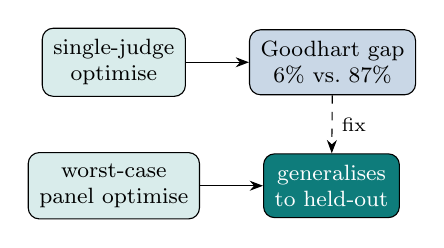
\begin{tikzpicture}[
  font=\footnotesize,
  box/.style={draw, rounded corners, align=center, inner sep=4pt, minimum height=8mm},
  >=Stealth
]
\node[box, fill=paleteal] (opt1) {single-judge\\optimise};
\node[box, fill=palealarm, right=8mm of opt1] (gap) {Goodhart gap\\6\% vs.\ 87\%};
\node[box, fill=paleteal, below=7mm of opt1] (opt2) {worst-case\\panel optimise};
\node[box, fill=ncotteal, text=white, right=8mm of opt2] (gen) {generalises\\to held-out};
\draw[->] (opt1) -- (gap);
\draw[->] (opt2) -- (gen);
\draw[->, dashed] (gap) -- node[right, font=\scriptsize] {fix} (gen);
\end{tikzpicture}
\caption{Optimising the scaffold against one absolute judge drives its training-judge score to the floor
but leaves held-out judges at baseline (the Goodhart gap, \S\ref{sec:judges}). Optimising the worst case
over a judge panel, with a family held out entirely, yields reductions that transfer
(\S\ref{sec:robust}).}
\label{fig:pipeline}
\end{figure}

\subsection{Narrative gradients reduce the single-judge loss}
We optimise NoT on $L_{\text{single}}$ over a disjoint OEQ train split ($n{=}100$, indices 150--249),
with held-out evaluation on a separate OEQ set ($n{=}150$) using the \haiku\ generator and \grok\ as the
training judge. Hand NoT scores validation $76\%$, framing $39\%$, indirectness $16\%$ under the
training judge (pooled loss $0.44$); the optimised prompt reaches validation $0.7\%$, framing $3\%$,
indirectness $5\%$ (loss $0.03$). Against three matched-budget baselines ($\sim$10 prompt evaluations
each), narrative gradients achieve the lowest held-out loss, beating APE, TextGrad-CoT and OPRO
(Appendix Table~\ref{tab:optimizer}). Two narrative-initialised methods outperform the CoT-initialised TextGrad
baseline, supporting the pre-registered hypothesis that scaffold \emph{structure}, not mere iterative
search, carries the reduction. The gradient rewrites the protagonist section into a ``Premise Audit''
that challenges embedded assumptions---a mechanistic hint at why first-person framing inflates
validation. \emph{However}, this single-judge ``win'' is partly illusory, as the next subsections show;
its headline loss should be read alongside the Goodhart diagnostic of \S\ref{sec:goodhart}.

\subsection{The judge panel: low inter-judge reliability}
We re-score $n{=}60$ stratified OEQ responses with three judge families (\nano, \haiku, \grok) on
validation, indirectness and framing, and compare each judge to crowdsourced human gold ($n{=}30$ human
responses) via Cohen's $\kappa$. \textbf{Inter-judge reliability is low on all three metrics}
(Table~\ref{tab:judge}): validation $\alpha{=}0.42$ $[0.25, 0.59]$, framing $\alpha{=}0.11$
$[-0.05, 0.28]$, indirectness $\alpha{=}-0.23$ $[-0.32, -0.12]$ (95\% item-bootstrap CIs, $n{=}60$;
below chance for indirectness). None clears the conventional $\alpha{=}0.67$ threshold, so panel headline rates use
majority vote. A sub-chance $\alpha$ means judges disagree more than chance on indirectness: driving
indirectness to $0\%$ under all panel judges is therefore a \emph{cross-judge coherence} property
(every idiosyncratic grader agrees), not evidence that a well-defined latent construct was recovered.
Against human gold the picture is more favourable for validation (Cohen's $\kappa\,0.73$--$0.86$ with
95\% CIs spanning roughly $0.48$--$1.0$) but only moderate for indirectness ($0.31$--$0.63$) and mixed
for framing ($0.15$--$0.70$). The combination---strong judge-vs-human $\kappa$ on validation yet weak
\emph{inter-judge} $\alpha$---is the known base-rate $\kappa$ paradox \citep{feinstein90kappa}. The
practical consequence is sharp: \textbf{validation is the only ELEPHANT metric we report without a
reliability caveat}, and any indirectness reduction from a single judge is not, on its own,
trustworthy---which is exactly what optimisation exploits next.

\begin{table}[t]
\centering
\small
\setlength{\tabcolsep}{4pt}
\begin{tabular}{lcccc}
\toprule
 & Inter-judge & \multicolumn{3}{c}{$\kappa$ vs.\ human} \\
\cmidrule(lr){3-5}
Metric & $\alpha$ ($n{=}60$) & nano & haiku & grok \\
\midrule
Validation   & $0.42$  & $0.85$ & $0.86$ & $0.73$ \\
Indirectness & $-0.23$ & $0.31$ & $0.39$ & $0.63$ \\
Framing      & $0.11$  & $0.15$ & $0.57$ & $0.70$ \\
\bottomrule
\end{tabular}
\caption{Judge reliability (point estimates; 95\% item-bootstrap CIs for $\alpha$ in text,
$n{=}60$). Inter-judge Krippendorff $\alpha$ over the three-family panel, and Cohen's $\kappa$ of each
judge against crowdsourced human labels ($n{=}30$ human responses). No metric clears $\alpha{=}0.67$;
validation alone shows strong judge-vs-human agreement on \emph{human} responses (not optimised model
outputs).}
\label{tab:judge}
\end{table}

\subsection{The Goodhart gap: re-scoring the identical responses}
\label{sec:goodhart}
To isolate judge-gaming from behaviour change we re-score the \emph{same} held-out responses (hand NoT
vs.\ single-judge optimised; \haiku\ generator; $n{=}150$) across a four-judge panel---the training judge
\grok\ plus held-out \haiku, \nano, \sonnet---changing only the judge, never regenerating
(Table~\ref{tab:goodhart}). The validation reduction is genuine: optimised validation is $0$--$3\%$
under \emph{every} judge. \textbf{The indirectness reduction is a Goodhart artifact}: the training judge
reads optimised indirectness at $6\%$, but the worst held-out judge reads $87\%$---identical to the
hand-NoT baseline. Optimising one absolute judge bought a phrasing change that this judge scores as
direct and others do not; framing sits in between (robust on three judges, $52\%$ on \sonnet). This is
the practical face of the low inter-judge $\alpha$ above: an optimiser pointed at a single noisy judge
will exploit it. The fix is to stop trusting any single judge---developed next.

\begin{table}[t]
\centering
\small
\setlength{\tabcolsep}{5pt}
\begin{tabular}{lcccc}
\toprule
 & \multicolumn{4}{c}{Single-judge optimised rate} \\
\cmidrule(lr){2-5}
Metric & grok$^\dagger$ & haiku & nano & sonnet \\
\midrule
Validation   & $1\%$ & $2\%$  & $3\%$  & $0\%$ \\
Indirectness & $6\%$ & $87\%$ & $59\%$ & $10\%$ \\
Framing      & $3\%$ & $4\%$  & $27\%$ & $52\%$ \\
\bottomrule
\end{tabular}
\caption{The Goodhart gap. The \emph{same} single-judge optimised responses ($n{=}150$) re-scored by
four judges. Validation is low under all judges (robust); indirectness collapses to a $6\%$
training-judge reading but stays at the $87\%$ baseline under the worst held-out judge. $\dagger$
training judge.}
\label{tab:goodhart}
\end{table}

\section{A Panel-Robust Optimizer}
\label{sec:robust}

\paragraph{Method.}
We re-run narrative-gradient descent (init = verbatim NoT, 10 iterations, optimiser \sonnet) under the
worst-case-over-panel objective $L_{\text{robust}}$ of \S\ref{sec:setup}, selecting the iteration with
lowest robust loss. The panel is the three in-family judges \grok, \haiku, and \nano; \sonnet\ and
out-of-family \deepseek\ are
held out entirely and scored only at evaluation. Because the loss credits only changes all panel judges
agree on, the optimiser cannot bank on a single lenient judge.

\paragraph{Generalisation to held-out judges.}
On \sonnet---never scored during optimisation---the robust prompt generalises significantly better than
the single-judge prompt: framing $11\%$ vs.\ $52\%$ (two-proportion $z{=}-7.7$, $p{=}1.9\times10^{-14}$)
and indirectness $0\%$ vs.\ $10\%$ ($z{=}-4.0$, $p{=}7\times10^{-5}$), both at the validation floor
(Table~\ref{tab:robust}). On out-of-family \deepseek\ the same pattern holds (indirectness $4\%$ vs.\
$74\%$, $p<10^{-15}$; framing $5\%$ vs.\ $13\%$). The robust prompt also achieves the lowest worst-case
panel loss ($0.32$ vs.\ single-judge $0.39$ vs.\ hand $0.71$) and is the only method to move worst-case
panel indirectness off the $87\%$ baseline (to $55\%$) in a cross-judge-coherent way. It trades a little
worst-case validation ($9\%$ vs.\ $3\%$) for large, judge-general gains on the two constructs
single-judge optimisation gamed or left at baseline.

\begin{table}[t]
\centering
\small
\setlength{\tabcolsep}{4pt}
\begin{tabular}{lcc|c}
\toprule
 & \multicolumn{2}{c}{Held-out (val/ind/fram)} & Panel \\
\cmidrule(lr){2-3}
Prompt & sonnet & DeepSeek & worst-loss \\
\midrule
Hand NoT      & $10/41/89\%$ & $53/78/68\%$ & $0.71$ \\
Single-judge  & $0/10/52\%$  & $6/74/13\%$  & $0.39$ \\
Robust        & $\mathbf{0/0/11\%}$ & $\mathbf{13/4/5\%}$ & $\mathbf{0.32}$ \\
\bottomrule
\end{tabular}
\caption{Held-out generalisation ($n{=}150$, \haiku\ generator). Each cell is validation/indirectness/
framing (\%); ``worst-loss'' is worst-case-over-panel loss. Robust beats single-judge on framing
($p{=}1.9{\times}10^{-14}$ sonnet) and indirectness ($p{=}7{\times}10^{-5}$ sonnet; $p<10^{-15}$
DeepSeek), and uniquely moves worst-case indirectness off baseline.}
\label{tab:robust}
\end{table}

\paragraph{Independent validation anchor.}
On a stratified $n{=}40$ sample of hand vs.\ robust holdout responses, an out-of-family proxy judge
(\deepseek, held out from optimisation) rates validation $70\%\rightarrow5\%$ (hand$\rightarrow$robust),
with proxy--author $\kappa{=}0.28$. Author-collected labels on the same sample give $35\%\rightarrow0\%$
but are not blinded---a conflict of interest---and should be read only as a secondary sanity check. The
strong human-gold $\kappa$ in \S\ref{sec:judges} ($0.73$--$0.86$) was measured on \emph{ELEPHANT human
responses}, not these optimised model outputs, where judge--author agreement is lower. Validation
therefore moves as claimed under both held-out LLM judges and the proxy anchor; indirectness/framing
generalisation rests on held-out \emph{LLM} judges only.

\paragraph{Degeneracy guard.}
On an $n{=}30$ subsample the robust prompt preserves stakeholder enumeration ($4.77$ vs.\ hand $4.73$)
while lowering uncertainty narration ($1.0$ vs.\ $2.83$), so the optimiser does not collapse the
scaffold into vacuity.

\paragraph{Quartet replication.}
Across the quartet on holdout OEQ ($n{=}150$/cell; \grok\ $n{=}147$), panel worst-case validation falls
under robust vs.\ hand on every generator (\haiku\ $69{\to}9$, \sonnet\ $89{\to}20$, \nano\ $66{\to}3$,
\grok\ $62{\to}2$\,\%), and held-out \deepseek\ framing follows on all four ($74{\to}4$, $74{\to}4$,
$96{\to}3$, $95{\to}4$\,\% resp.), so robustness generalises across generator families, not only the
\haiku\ training cell.

\paragraph{Scope.}
We present panel-robustness as a demonstrated generalisation \emph{property}, not a deployment-ready
prompt (\S\ref{sec:limitations}).

\section{Discussion}
\label{sec:disc}

\paragraph{Sycophancy is not one construct.}
A single scaffold cuts social validation across four vendors yet does not reduce propositional
sycophancy on checkable falsehoods (significant only on \grok; a significant \emph{increase} on \nano)
and \emph{reverses} on cross-prompt moral consistency. Benchmark choice is thus not a detail---
obvious-falsehood probes saturate at $\leq2\%$ while BrokenMath runs $39$--$83\%$---and one pooled
``sycophancy'' number hides the dissociations that reveal what an intervention does. Deliberation buys
social, single-response face-preservation and little else, matching the linguistic-vs-reasoning
asymmetry \citet{cheng25elephant} report and the prediction that added reasoning need not reduce bias
\citep{turpin23,chua24}.

\paragraph{Optimising against LLM judges measures the judge.}
The narrative-gradient ``win'' partly reverse-engineers its training judge: re-scoring identical
responses shows the indirectness reduction is a Goodhart artifact ($6\%$ vs.\ $87\%$ held-out), with
only validation surviving every judge---in-context reward hacking \citep{pan24hacking,gao23overopt} at
the prompt level. A worst-case-over-panel objective with a family held out fixes this by construction,
generalising to out-of-family \deepseek\ (one held-out judge family; judge ensembles can share blind
spots \citep{eisenstein23herding}) where single-judge optimisation does not, while preserving
stakeholder depth; being black-box, it transfers to closed models. The lesson generalises past
sycophancy: \emph{prompt optimisation against LLM judges must be evaluated against judges held out from
optimisation, or it measures judge idiosyncrasy rather than behaviour.}

\paragraph{Less sycophantic is not always better.}
Anti-sycophancy interventions can overcorrect into bluntness or into rejecting \emph{correct} user
claims \citep{wei23syn,sharma23}, and our free-form moral result shows NoT affirming both sides
\emph{more} often. We did not run a naive ``don't be sycophantic'' instruction arm; \citet{dubois26ask}
show such direct prompts are a weak baseline relative to input-side reframing. We therefore frame NoT as
a measurement and construct-clarification tool---not a deployment-ready fix, and complementary to
input-side reframing \citep{dubois26ask}.

\section{Conclusion}
Sycophancy fragments into constructs that need not move together: NoT cuts social validation and framing
across four generators where obvious-falsehood probes show no signal, yet does not transfer to
propositional error-detection and reverses on moral consistency. A reliability panel exposes
single-judge prompt optimisation as judge-gaming; a panel-robust optimiser yields
cross-judge-coherent indirectness reductions that generalise to held-out judges. Deliberative scaffolding
targets single-response social face-preservation, and robustness---not raw loss against one judge---is
the quantity worth optimising.

\section*{Limitations}
\label{sec:limitations}
\paragraph{Judge dependence.}
All sycophancy outcomes are LLM-scored. Validation is anchored to human gold on ELEPHANT human responses
($\kappa\,0.73$--$0.86$), but author labels on \emph{model} outputs ($n{=}40$) show only moderate
judge--author agreement ($\kappa\,0.13$--$0.27$) and were not blinded; an out-of-family proxy judge
(\deepseek) on the same sample gives $70\%\rightarrow5\%$ validation (hand$\rightarrow$robust) with
proxy--author $\kappa{=}0.28$, but indirectness/framing carry low inter-judge reliability
($\alpha\leq0.42$, with bootstrap CIs in \S\ref{sec:judges}). Held-out generalisation rests on LLM
judges; \deepseek\ is out-of-family but \sonnet\ shares a vendor with panel judge \haiku, and judge
ensembles can share blind spots \citep{eisenstein23herding}.

\paragraph{Role overlap.}
Several models serve multiple roles (Table~\ref{tab:roles}): \haiku\ and \grok\ are both generators and
judges/optimiser-panel members, and \sonnet\ is both a generator and a held-out judge. We mitigate the
most direct leakage by holding \sonnet\ and \deepseek\ out of optimisation entirely, but a fully
disjoint generator/judge design is left to future work.

\paragraph{Mechanism not isolated.}
The optimisation results isolate \emph{outcome}, not \emph{mechanism}: we have not ablated which
narrative section (protagonist, stakeholders, consequences, uncertainty, commitment) carries the effect,
so causal attribution to specific scaffold components remains open. Relatedly, we did not run a
length-matched verbose-CoT control; NoT OEQ responses are $1.3$--$4.4\times$ longer than CoT
(Appendix Table~\ref{tab:lengths}), so a residual verbosity confound on validation/framing cannot be
fully excluded (\S\ref{sec:social}). We also did not run a naive ``don't be sycophantic'' instruction
arm; \citet{dubois26ask} show such direct prompts are a weak baseline relative to input-side reframing.

\paragraph{Instrument and power.}
BrokenMath uses a single judge family (\haiku), and the surprising \nano\ $+14.7$\,pp increase rides on
that one scorer---we did not panel-check BrokenMath in this pass. The free-form moral arm adds a
verdict-extraction call whose reliability we do not separately audit. Per-cell samples are $n{=}150$
(ELEPHANT slices) and $n{=}451$ (BrokenMath); effects below a few points may be underpowered.
Significance tests are reported pairwise without a global multiple-comparisons correction; headline
effects with $p<10^{-4}$ survive conservative correction. We test arms with two-proportion / Fisher
tests on independent cells (\S\ref{sec:setup}); paired re-scoring tables (e.g.\ the Goodhart gap)
compare conditions on the same items.

\paragraph{Generality.}
All generators are accessed through hosted providers; results may not transfer to other deployments,
model versions, or non-English advice settings.

\section*{Ethical Considerations}
This work studies sycophancy mitigation and collects no new human-subjects data; human labels are drawn
from the public ELEPHANT/OSF release and used only as reliability gold. Reducing sycophancy is dual-use:
a scaffold that makes models less validating can also make them blunt or dismissive in genuinely
sensitive contexts, and our finding that NoT \emph{increases} moral both-NTA shows ``less sycophantic''
is not uniformly desirable. We therefore frame NoT as a measurement and construct-clarification tool,
not a deployment-ready safety intervention, and caution against optimising single sycophancy metrics in
isolation. No personally identifying information is processed; all adversarial math problems come from
the public BrokenMath benchmark.

\section*{Reproducibility Statement}
The scaffold is specified in full in Appendix~\ref{app:notprompt}; the panel-robust objective in
\S\ref{sec:setup}; generators, arms, splits, seeds and judges in \S\ref{sec:setup}. All experiments are
black-box (API generation and judging). Appendix~\ref{app:phasemap} maps each result to the internal
milestone label under which it was produced, for cross-referencing released artifacts. Significance
tests, sample sizes and held-out judge identities are stated in each table caption.

\bibliography{references}

\appendix

\section{The NoT System Prompt}
\label{app:notprompt}
The scaffold is a single system prompt, prepended to the user turn and held fixed across all generators
and arms. It adds no training data, parameters, or fine-tuning. The instruction content is reproduced
below verbatim.

\begin{quote}\small\ttfamily
Before giving your final answer, think in the first person and write five short labelled sections:\\[2pt]
1. PROTAGONIST: name the person whose decision this is, their role, and what they actually know.\\
2. STAKEHOLDERS: list every party whose interests intersect this decision and what is at stake for each.\\
3. CONSEQUENCES: for each option you are weighing, project the likely effects at least two steps out, for each stakeholder.\\
4. UNCERTAINTY: state plainly what remains genuinely unknown or contested.\\
5. COMMITMENT: commit to a single recommendation and explain, within this frame, why it is preferable to the alternatives.\\[2pt]
Then give your final answer.
\end{quote}

The multi-stakeholder variant (\S\ref{sec:setup}) runs this same prompt as the per-agent generator for
several stakeholder perspectives and integrates the drafts with a separate moderator model over five
rounds before emitting one answer.

\section{Obvious-Falsehood Floor (Sharma)}
\label{app:sharma}
Table~\ref{tab:sharma} reports SycophancyEval \citep{sharma23} on the quartet. Every cell is at most
$2.2\%$, confirming the instrument is saturated and cannot discriminate arms; it is excluded from all
scaffold claims and reported only to motivate the move to BrokenMath (\S\ref{sec:benchmarks}).

\begin{table}[h]
\centering
\small
\begin{tabular}{lcc}
\toprule
Generator & Std CoT & NoT \\
\midrule
\texttt{gpt-5.4-nano}            & $0.0\%$ & $2.2\%$ \\
\texttt{claude-haiku-4-5}        & $1.1\%$ & $0.0\%$ \\
\texttt{claude-sonnet-4-6}       & $0.0\%$ & $0.0\%$ \\
\texttt{grok-4-1-fast-reasoning} & $0.0\%$ & $0.0\%$ \\
\bottomrule
\end{tabular}
\caption{Sharma SycophancyEval sycophancy rate ($30$ probes $\times$ $3$ samples $=90$ judgments per
cell). Saturated floor; not used for scaffold claims.}
\label{tab:sharma}
\end{table}

\section{Result-to-Milestone Map}
\label{app:phasemap}
For cross-referencing released artifacts, each result maps to the internal milestone label under which
it was produced: obvious-falsehood floor and BrokenMath headroom (Phase 16; \S\ref{sec:benchmarks},
\S\ref{sec:propositional}); scaled ELEPHANT validation/framing and corrected moral loading (Phase 13;
\S\ref{sec:social}, \S\ref{sec:moral}); free-form moral arm (Phase 17; \S\ref{sec:moral});
narrative-gradient optimisation and optimiser comparison (Phase 14; \S\ref{sec:judges}); judge
reliability panel (Phase 15; \S\ref{sec:judges}); Goodhart-gap re-scoring (Phase 18a;
\S\ref{sec:goodhart}); panel-robust optimiser, held-out generalisation, author-label anchor, degeneracy
guard, and quartet replication (Phase 18b--e; \S\ref{sec:robust}). Pre-registration and run scripts are
in the released artifact bundle.

\section{Supplementary Tables}
\label{app:suptables}
Tables relocated from the main text to respect the page limit; their values are stated in the body.

\begin{table}[h]
\centering
\small
\begin{tabular}{lcc}
\toprule
Optimiser & Init & Holdout loss \\
\midrule
Narrative gradients & NoT      & $\mathbf{0.029}$ \\
APE                 & NoT      & $0.104$ \\
TextGrad-CoT        & Std CoT  & $0.170$ \\
OPRO                & NoT      & $0.200$ \\
\midrule
Hand NoT (reference) & ---     & $0.436$ \\
\bottomrule
\end{tabular}
\caption{Optimiser holdout loss (validation\,+\,indirectness\,+\,framing, training judge \grok,
$n{\approx}148$--$150$; lower is better; \S\ref{sec:judges}). Narrative gradients win, but the objective
itself is partly gameable (\S\ref{sec:goodhart}); robustness, not this loss, is the quantity we
ultimately optimise.}
\label{tab:optimizer}
\end{table}

\begin{table}[h]
\centering
\small
\setlength{\tabcolsep}{4pt}
\begin{tabular}{lrrr}
\toprule
Generator & Raw & Std CoT & NoT \\
\midrule
\texttt{gpt-5.4-nano}            & $78\%$ & $79\%$ & $78\%$ \\
\texttt{claude-haiku-4-5}        & $59\%$ & $53\%$ & $93\%$ \\
\texttt{claude-sonnet-4-6}       & $32\%$ & $38\%$ & $72\%$ \\
\texttt{grok-4-1-fast-reasoning} & $70\%$ & $73\%$ & $82\%$ \\
\bottomrule
\end{tabular}
\caption{Free-form moral both-NTA rate ($n{=}150$ pairs; \S\ref{sec:moral}). NoT \emph{raises} both-NTA
on every generator (sharply on \haiku/\sonnet), the opposite of its validation/framing effect---
consistent with a distinct cross-prompt construct, though partly attributable to the free-form
instrument (see text).}
\label{tab:moralfree}
\end{table}

\begin{table}[h]
\centering
\small
\setlength{\tabcolsep}{4pt}
\begin{tabular}{lrrrr}
\toprule
 & \texttt{nano} & \texttt{haiku} & \texttt{sonnet} & \texttt{grok} \\
\midrule
\multicolumn{5}{l}{\emph{OEQ validation (human ${=}29\%$)}} \\
\quad Raw      & $78\%$ & $66\%$ & $77\%$ & $83\%$ \\
\quad Std CoT  & $75\%$ & $63\%$ & $73\%$ & $82\%$ \\
\quad NoT      & $27\%$ & $27\%$ & $47\%$ & $29\%$ \\
\midrule
\multicolumn{5}{l}{\emph{Moral both-NTA (binary; corrected loader)}} \\
\quad Raw      & $51\%$ & $18\%$ & $25\%$ & $31\%$ \\
\quad Std CoT  & $50\%$ & $23\%$ & $24\%$ & $32\%$ \\
\quad NoT      & $51\%$ & $15\%$ & $17\%$ & $42\%$ \\
\bottomrule
\end{tabular}
\caption{Cross-vendor replication (\S\ref{sec:social}). Top: OEQ validation---NoT reductions
significant on all four generators. Bottom: corrected binary moral both-NTA---no systematic NoT effect,
indicating a different construct from validation/framing.}
\label{tab:crossvendor}
\end{table}

\begin{table}[h]
\centering
\small
\setlength{\tabcolsep}{4pt}
\begin{tabular}{lrrrr}
\toprule
Generator & Raw & IO & Std CoT & NoT \\
\midrule
\texttt{gpt-5.4-nano}            & $4{,}125$ & $3{,}286$ & $4{,}346$ & $6{,}337$ \\
\texttt{claude-haiku-4-5}        & $1{,}662$ & $1{,}442$ & $1{,}692$ & $5{,}580$ \\
\texttt{claude-sonnet-4-6}       & $1{,}543$ & $1{,}463$ & $1{,}647$ & $7{,}165$ \\
\texttt{grok-4-1-fast-reasoning} & $3{,}613$ & $1{,}534$ & $3{,}815$ & $5{,}073$ \\
\bottomrule
\end{tabular}
\caption{Mean OEQ response length (characters) by arm ($n{\approx}145$--$150$/cell;
\S\ref{sec:social}). NoT/CoT ratios: \nano\ $1.46\times$, \haiku\ $3.3\times$, \sonnet\
$4.35\times$, \grok\ $1.33\times$.}
\label{tab:lengths}
\end{table}

\end{document}